\documentclass[../main.tex]{subfiles}

\begin{document}
Two main problems of calculus are
\begin{enumerate}
  \item Derivative. Find the rate of change of $f$.
  \item Integral. Find the area under a given curve.
\end{enumerate}
Both are based on the concept of limit.

We say $\lim_{x \to a} f(x) = L$ to mean that $f(x)$ is ``close enough'' to $L$ when $x$ is ``close enough'' to \emph{but not equal to} $a$. Hence $f(a)$ is unimportant for $\lim_{x \to a} f(x)$.

\begin{example}
  Which value is $x$ close to when $x$ is close to 2? $\lim_{x \to 2} x = 2$.
\end{example}

\begin{example}
  Which value is 3 close to when $x$ is close to 2? $\lim_{x \to 2} 3 = 3$.
\end{example}

We can generalize these examples.
\begin{theorem}
\label{basic limit theorems}
  Let $a$ and $c$ be two real numbers. Then
  \[
    \lim_{x \to a} c = c, \qquad
    \lim_{x \to a} x = x.
  \]
\end{theorem}


The limit $\lim_{x \to a} f(x)$ may be different from $f(a)$ as the next example shows.
\begin{example}
  \[
    f(x) =
    \begin{cases}
      x, &\text{ if } x\neq 2\\
      1, &\text{ if } x = 2\\
    \end{cases}
  \]
  Which value is $f(x)$ close to when $x$ is close to (but not equal to) 2?

  $\lim_{x \to 2} f(x) = \lim_{x \to 2} x = 2$ although $f(2) = 1$.
\end{example}

\subsection*{Informal definition of left and right limits}
If $f(x)$ is close to $L$ when $x<a$ and $x$ is close enough to $a$ then we say
\[
  \lim_{x \to a^{-}} f(x) = L
\]
This is called the \emph{left limit} of $f$ at $x=a$.

Similarly we can define the right limit.

\begin{theorem}
  $\lim_{x \to a} f(x) = L$ if and only if both $\lim_{x \to a^{-}} f(x) =L$ and $\lim_{x \to a^{+}} f(x) = L$.
\end{theorem}

\begin{example}
Find the left and right limits of the signum function

  \begin{minipage}[c]{0.5\textwidth}
    \[
    f(x) =
    \begin{cases}
      -1 & \text{for $x<0$}\\ 0 & \text{for $x=0$}\\ 1 & \text{for $x>0$}
    \end{cases}
    \]
  \end{minipage}
  \begin{minipage}[c]{0.2\textwidth}
    \begin{figure}[H]
    \centering
    \begin{tikzpicture}
  \draw [<->] (-1.5,0) -- (1.5,0);
  \draw [<->] (0,-1.5) -- (0,1.5);
  \draw [thick, blue] (-1,-1) -- (0,-1);
  \draw [thick, blue] (1,1) -- (0,1);
  \node[left] at (0,1) {$1$};
  \node[right] at (0,-1) {$-1$};
  \draw[fill=blue] (0, 0) circle [radius=.1];
  \draw[fill=white] (0, -1) circle [radius=.1];
  \draw[fill=white] (0, 1) circle [radius=.1];
\end{tikzpicture}
    \end{figure}
  \end{minipage}

  In this example the one-sided limits exist, but are not equal
  \[
  \lim_{x\searrow0}f(x) = 1 \text{ and } \lim_{_x\nearrow0}f(x) = -1.
  \]
  Hence $\lim_{x\to 0} f(x)$ does not exist.
\end{example}


% \begin{example} Evaluate the expressions by referencing the plot in Figure~\ref{plot:piecewise-exercise}.
% \begin{figure}[H]
%   \centering
%   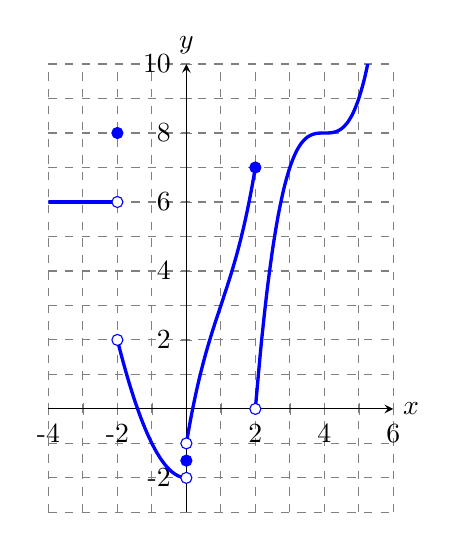
\begin{tikzpicture}
  \begin{axis}[
            domain=-4:6, xmin=-4, xmax=6, ymin=-3,ymax=10,
            unit vector ratio*=1 1 1,
            axis lines =middle, xlabel=$x$, ylabel=$y$,
            every axis y label/.style={at=(current axis.above origin),anchor=south},
            every axis x label/.style={at=(current axis.right of origin),anchor=west},
            xtick={-4,...,6}, ytick={-3,...,10},
            xticklabels={-4,,-2,,0,,2,,4,,6}, yticklabels={,-2,,0,,2,,4,,6,,8,,10},
            grid=major,
            grid style={dashed, gray},
          ]
    \addplot [very thick, blue, smooth, domain=(-4:-2)] {6};
    \addplot [very thick, blue, smooth, domain=(-2:0)] {x^2-2};
          \addplot [very thick, blue, smooth, domain=(0:2)] {(x-1)^3+3*(x-1)+3};
          \addplot [very thick, blue, smooth, domain=(2:6)] {(x-4)^3+8};
          \addplot[color=blue,fill=white,only marks,mark=*] coordinates{(-2,6)};  %% open hole
          \addplot[color=blue,fill=white,only marks,mark=*] coordinates{(-2,2)};  %% open hole
          \addplot[color=blue,fill=white,only marks,mark=*] coordinates{(0,-2)};  %% open hole
          \addplot[color=blue,fill=white,only marks,mark=*] coordinates{(0,-1)};  %% open hole
          \addplot[color=blue,fill=white,only marks,mark=*] coordinates{(2,0)};  %% open hole
          \addplot[color=blue,fill=blue,only marks,mark=*] coordinates{(-2,8)};  %% closed hole
          \addplot[color=blue,fill=blue,only marks,mark=*] coordinates{(0,-1.5)};  %% closed hole
          \addplot[color=blue,fill=blue,only marks,mark=*] coordinates{(2,7)};  %% closed hole
        \end{axis}
\end{tikzpicture}
%   \label{plot:piecewise-exercise}
% \end{figure}

% \begin{enumerate}
% \begin{multicols}{3}
% \item $\lim_{x\to 4} f(x)$
% \item $\lim_{x\to -3} f(x)$
% \item $\lim_{x\to 0} f(x)$
% \item $\lim_{x\to 0-} f(x)$
% \item $\lim_{x\to 0+} f(x)$
% \item $f(-2)$
% \item $\lim_{x\to 2-} f(x)$
% \item $\lim_{x\to -2-} f(x)$
% \item $\lim_{x\to 0} f(x+1)$
% \item $f(0)$
% \item $\lim_{x\to 1-} f(x-4)$
% \item $\lim_{x\to 0+} f(x-2)$
% \end{multicols}
% \end{enumerate}

% (a) $8$, (b) $6$, (c) DNE,
% (d) $-2$, (e) $-1$, (f) $8$,
% (g) $7$, (h) $6$, (i) $3$,
% (j) $-3/2$, (k) $6$, (l) $2$
% \end{example}

\subsection*{Properties of Limits}
\begin{theorem}
  Suppose
  \[
  \lim_{x\to a}f(x)=L, \qquad \lim_{x\to a}g(x)=M.
  \]
  Then
  \begin{align}
    & \lim_{x\to a}\bigl(f(x)+g(x)\bigr)=L+M,  \\
    & \lim_{x\to a}\bigl(f(x)-g(x)\bigr)= L - M,  \\
    & \lim_{x\to a}\bigl(f(x)\cdot g(x)\bigr)= L\cdot M \\
    & \lim_{x\to a}\frac{f(x)}{g(x)}= \frac{L}{M}, \quad \text{if } M \neq 0.
  \end{align}
  Finally, if $m$ and $n$ are integers such that $L^{m/n}$ is defined
  \begin{equation}
    \lim_{x\to a}(f(x))^{m/n}= L^{m/n}.
  \end{equation}
\end{theorem}

Using the above properties we can evaluate the following limits.
\begin{example}
  Find $\lim_{x \to 2} x^2 +1$ and $\lim_{x \to 2} \dfrac{x^2+1}{6-x}$.

  Solution. Using the product rule of limits and the Theorem~\ref{basic limit theorems},
  \[
    \lim_{x \to 2} x^2 = \lim_{x \to 2} x \cdot \lim_{x \to 2} x = 2 \cdot 2 = 4
  \]
  Using the sum rule of limits,
  \[
    \lim_{x \to 2} x^2 + 1= \lim_{x \to 2} x^2 + \lim_{x \to 2} 1 = 4 + 1 = 5
  \]
  Using the division rule of limits,
  \[
    \lim_{x \to 2} \frac{x^2+1}{6-x} = \frac{\lim_{x \to 2} x^2+1}{\lim_{x \to 2} 6-x} = \frac{5}{4}.
  \]
\end{example}

The above example is a special case of the following theorem.
\begin{theorem}
  If $P(x)$ is a polynomial then,
  \[
    \lim_{x \to a} P(x) = P(a)
  \]
  If $Q(x)$ is another polynomial with $Q(a) \neq 0$ then
  \[
    \lim_{x \to a} \frac{P(x)}{Q(x)} = \frac{P(a)}{Q(a)}.
  \]
\end{theorem}

\subsection*{The Squeeze Theorem}

\begin{theorem}
  Suppose that $f(x) \le g(x) \le h(x)$ and $\lim_{x \to a} f(x) = \lim_{x \to a} h(x) = L$. Then $\lim_{x \to a} g(x) = L$.
  \begin{figure}[H]
    \centering
    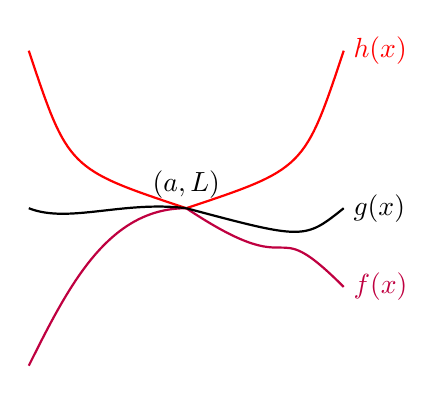
\begin{tikzpicture}[scale=1]
  \draw[purple, thick] (-2,-2) .. controls (-1.5,-1) and (-1,0) .. (0,0);
  \draw[purple, thick] (0,0) .. controls (1.5,-1) and (1,0) .. (2,-1);

  \draw[red, thick] (-2,2) .. controls (-1.5,.5) .. (0,0);
  \draw[red, thick] (0,0) .. controls (1.5,.5) .. (2,2);

  \draw[black, thick] (-2,0) .. controls (-1.5,-.2) and (-.8, .1) .. (0,0);
  \draw[black, thick] (0,0) .. controls (1.5,-.4) .. (2,0);
  \node[right, red]  at (2,2) {$h(x)$};
  \node[right, purple]  at (2,-1) {$f(x)$};
  \node[right, black]  at (2,0) {$g(x)$};
  \node[above] at (0, 0) {$(a, L)$};
\end{tikzpicture}
    \caption{The Squeeze Theorem.}
  \end{figure}
\end{theorem}

\begin{example}
  If $2-x^2 \le g(x) \le 2 \cos x$ for $-1\le x \le 1$, find $\lim_{x \to 0}f(x)$.
\end{example}

\begin{example}
  Show that if $\lim_{x \to a} \abs{f(x)} = 0$ then $\lim_{x \to a} f(x) = 0$.

  Note that $-\abs{f(x)} \le f(x) \le \abs{f(x)}$ and use the Squeeze Theorem.
\end{example}

\subsection*{More examples}
\begin{example}
  Let
  \[
    f(x) = \frac{\abs{x-2}}{x^2+x-6}.
  \]
  Find $\lim_{x \to 2+} f(x)$, $\lim_{x \to 2-} f(x)$. Does $\lim_{x \to 2} f(x)$ exist?
\end{example}

In these example, we will compute $\lim_{x \to a} f(x)$ even when $f(a)$ does not exist.
\begin{example}
  Evaluate
  \begin{enumerate}
    \item $\lim_{x \to -2} \dfrac{x^2 + x-2}{x^2 + 5x +6}$,

    \textit{Remember} that we consider $x$ values close to but not equal to $-2$. Hence $x+2 \neq 0$ and we can make the simplification
    \[
      \lim_{x \to -2} \dfrac{x^2 + x-2}{x^2 + 5x +6} =
      \lim_{x \to -2} \dfrac{(x+2)(x-1)}{(x+2)(x+3)} =
      \lim_{x \to -2} \dfrac{x-1}{x+3} = \frac{-3}{1} = -3.
    \]
    \item $\lim_{x \to 5} \dfrac{\frac{1}{x} - \frac{1}{5}}{x-5}$,
    \item $\lim_{x \to 4} \dfrac{\sqrt{x}-2}{x^2-16}$,

    \textit{Trick} is to multiply both sides by the conjugate expression.
    \item $\lim_{x \to -2} \dfrac{x^2 + 2x}{x^2-4}$,
    \item $\lim_{h \to 0} \dfrac{\sqrt{4+h}-2}{h}$,
    \item $\lim_{t \to 0} \dfrac{t}{\sqrt{4+t}-\sqrt{4-t}}$,
    \item $\lim_{x \to -1} \dfrac{x^3+1}{x+1}$,
    \item $\lim_{x \to 0} \dfrac{\abs{3x-1}-\abs{3x+1}}{x}$,
    \item $\lim_{x \to 2-} \dfrac{x^2-4}{\abs{x+2}}$.
  \end{enumerate}
\end{example}
\end{document}